% Appendix: does not count toward the page limit.

\section{Training and inference details}
\label{app:training}
All 2D models were trained with an equally weighted sum of binary cross-entropy and Dice loss, AdamW (learning rate $10^{-4}$, no weight decay), a cosine schedule, at most 100 epochs and mixed precision, with batch size 8 (4 for SwinUNETR). Input size was $352\times352$. Training augmentation was a random rotation by a multiple of 90$^\circ$, horizontal and vertical flips (each $p=0.5$), and brightness and contrast scaling by factors in $[0.85, 1.15]$ on the raw image. Pretrained encoders used ImageNet normalisation and SwinUNETR used per-fold dataset statistics. We kept the checkpoint with the best Dice on the validation fold and stopped after 20 epochs without improvement. The test fold was never used during training or selection.

The 3D SegResNet used the four MRI sequences (FLAIR, T1, T1-Gd, T2), each clipped at its 1st and 99th brain percentiles and z-scored over brain voxels. Training used the same loss, optimiser and schedule, $128^3$ patches from the brain bounding box, 90\% of them centred on an enhancing-tumour voxel (250 per epoch), at most 100 epochs with patience 20 on Dice over 40 validation-fold patients, and flips on all three axes, axial 90$^\circ$ rotations and intensity jitter of $\pm0.1$ as augmentation. Inference used sliding windows of $128^3$ with overlap 0.5 and Gaussian weighting.

We measured per-pass latency on a laptop GPU (NVIDIA RTX 4050, batch 1, mixed precision, $352\times352$): 10 warm-up passes, then the median of three blocks of 50 passes. TTA latency is estimated as passes times the per-pass median.


The six uncertainty signals of Section~\ref{sec:eval} are: the mean predictive entropy in the ROI for the single view and for the TTA-4 mean map, the mean TTA-4 variance in the ROI, one minus the mean probability inside the predicted mask, the fraction of pixels on which the binarised views do not all agree, and one minus the mean pairwise Dice between views. The ROI is the predicted foreground plus a 3-pixel band around it. The third failure definition compares empty predictions against clean cases, meaning non-empty predictions with Dice at least 0.5.

\paragraph{Statistical detail from Section~\ref{sec:eval}.} Bootstrap intervals use 10{,}000 draws, reduced to 2{,}000 for between-model gain comparisons and MC-Dropout and 1{,}000 for the uncertainty audit and its paired tests. External rates of empty predictions carry Jeffreys intervals. For tails we report the 90th percentile of HD95 and the large-failure rate with bootstrap intervals of the change. Gains across models are compared as the absolute change, the share of remaining error recovered ($\Delta\mathrm{Dice}/(1-\mathrm{Dice}_{\text{base}})$, computed per video then averaged) and the log ratio of HD95; because a plain correlation between baseline error and gain is biased by regression to the mean, we use Oldham's method \cite{oldham1962} against a permutation null that exchanges baseline and TTA scores within whole videos. Counts per checkpoint are descriptive.

\section{Further internal comparisons}
\label{app:further}
% Source: aggregate_*/ensemble_comparison.csv; mc_dropout_cvc_clinicdb_unet_resnet50_dropout/deltas.csv.
\paragraph{Large failures and the extreme tail (internal).} TTA-4 cut the share of frames with HD95 above 50\,px, or with no prediction from any seed, from 41.0\% to 31.0\% for UNet (95\% CI $[-15.0, -5.4]$ points) and from 27.8\% to 25.7\% for SegFormer, while neither 90th percentile of HD95 moved reliably ($-10.3$\,px $[-25.4, 2.3]$ and $-4.0$\,px $[-14.4, 11.4]$). For SwinUNETR and BraTS the upper tail did shrink, by 9.0\,px $[-14.6, -1.4]$ and 1.5\,mm $[-3.0, -0.3]$, and on BraTS large failures fell from 11.9\% to 10.7\% $[-2.1, -0.3]$. HD95 percentiles use each method's own non-empty cases.

A three-seed deep ensemble was not significantly better than TTA-4 of a single model. The Dice difference was +0.003 for UNet, +0.004 for SegFormer and +0.006 for SwinUNETR, with Holm $p=1.0$ in each case. Combining the two added 0.013, 0.007 and 0.018 Dice over TTA-4 ($p<0.001$). MC-Dropout with eight passes was, if anything, slightly worse than the deterministic pass of the same network (Dice $-0.001$, unadjusted 95\% CI $[-0.002, -0.0001]$, Holm $p=0.13$) and stayed 0.022 below TTA-4 of that network (Holm $p<0.001$).

% Source: compare_data_sweep/deltas.csv and gain_difference.csv (seed 0 only); compare_models/residual_error.csv.
% Source: compare_models/gain_difference.csv (TTA-4, paired by video, unadjusted p); compare_models/residual_error.csv.
In absolute Dice, the two weaker models gained numerically more than the strongest: UNet (+0.023) gained more than the stronger SegFormer (+0.011; difference 0.012, 95\% CI $[0.003, 0.021]$, $p=0.002$) and about as much as the weaker SwinUNETR (+0.021; $p=0.37$). Relative to what was left to gain, the mid-quality UNet gained most. As a share of the remaining error, computed per video and then averaged so that it differs from the ratio of the means in Table~\ref{tab:internal}, UNet closed 13.0\%, SegFormer 7.1\% and SwinUNETR 6.3\%, and UNet's share was larger than both ($p=0.004$ and $p=0.006$). HD95 followed the same pattern on a log scale: $-0.39$ for UNet against $-0.11$ for both other models ($p<0.001$).

Within UNet, less training data did not raise the gain. With 100\%, 50\% and 25\% of the training videos (5 folds at one seed, so the 100\% arm's 0.028 is not Table~\ref{tab:internal}'s 0.023), TTA-4 added 0.028, 0.026 and 0.014 Dice; the last was not significant (Holm $p=0.07$), and no two fractions differed in Dice gain ($p\geq0.55$). Within each model, harder cases did not consistently gain more. With Oldham's correction, the correlation between a case's mean score and its Dice gain was $-0.11$ for UNet (permutation $p=0.16$), $-0.15$ for SegFormer ($p=0.08$) and $+0.17$ for SwinUNETR ($p=0.04$), where it was the better cases that gained more.

The workshop study reported larger TTA gains for a lower-performing model \cite{kashyap2026unsure}, based on one model trained from scratch against pretrained ones and without relating baseline error to gain. Here the mid-quality UNet gained more than the stronger SegFormer (0.023 against 0.011, $p=0.002$), and the weaker SwinUNETR did not gain significantly more than UNet (0.021, $p=0.37$) and recovered a smaller share of its error. The workshop UNet showed no Dice gain ($-0.005$), while the retrained UNet here gains 0.023, so the two studies are not directly comparable.


\section{Additional result figures}
\label{app:figs}

\begin{figure}[htbp]
\floatconts
  {fig:misses}
  {\caption{Empty predictions without TTA, with TTA-4 and with TTA-8 (grey shades). (a) Internal: share of cases with an empty prediction (CVC-ClinicDB frames empty in at least 2 of 3 seeds; BraTS patients), with 95\% cluster-bootstrap intervals and Holm-adjusted McNemar $p$. (b) UNet and (c) SegFormer on the external sets: share of images left empty by at least 8 of 15 checkpoints, with 95\% Jeffreys intervals and exact McNemar $p$ (unadjusted). SwinUNETR left no external image empty by majority. No-overlap and missed counts are in Table~\ref{tab:external}.}}
  {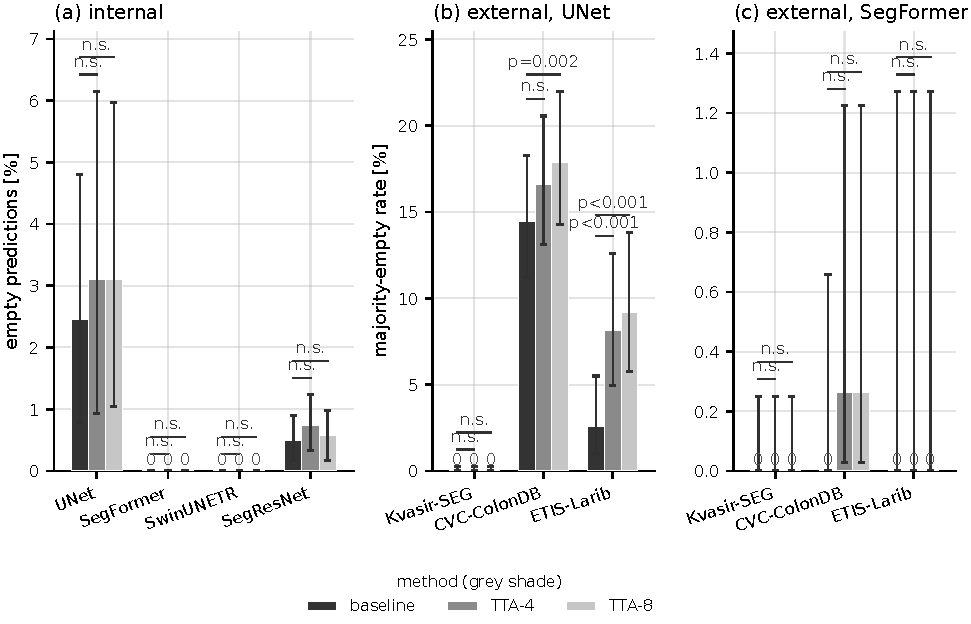
\includegraphics[width=\linewidth]{figures/fig03_misses.pdf}}
\end{figure}

These figures show results that the main text reports in numbers: the risk--coverage curves of Section~\ref{sec:res-uncertainty} (Fig.~\ref{fig:riskcov}), the gain against the number of views of Section~\ref{sec:res-internal} (Fig.~\ref{fig:views}), the HD95 distribution of Section~\ref{sec:res-failures} (Fig.~\ref{fig:ecdf}) and the gain against domain gap of Section~\ref{sec:res-external} (Fig.~\ref{fig:external}).

Three further numbers from the uncertainty audit of Section~\ref{sec:res-uncertainty}. On BraTS the TTA-4 variance in the ROI was the best signal (AUROC 0.96, against 0.90 for ROI entropy, $p<0.002$), while view disagreement ranked failures there as more certain than successes (0.36). Pairwise Dice between views, computed for UNet only, scored higher than view disagreement on the empty frames (0.71 against 0.21, 19 frames), but its 95\% CI $[0.50, 0.95]$ reaches chance.

Why view disagreement fails on empty predictions: an empty prediction has almost no pixels on which views can disagree, because the score of Section~\ref{sec:eval} is a fraction of all image pixels and is not normalised by predicted area, while the boundary of a large, correctly segmented lesion adds many pixels. A version normalised by predicted area plus band would be the natural repair, and it needs no retraining; we did not compute one, so we report the defect rather than a fix.

\begin{figure}[htbp]
\floatconts
  {fig:riskcov}
  {\caption{Risk--coverage curves of five uncertainty signals, UNet on CVC-ClinicDB, each scored against the failures of its own prediction: (a) Dice $<0.5$ on a non-empty prediction, (b) the same plus empty predictions; ROI-based signals are undefined on the 14 frames with no prediction from any seed and exclude them. Cases are kept from the most confident; the curve shows the failure rate of the kept cases. The two numbers after each signal in the legend are its AUROC and its AURC, the latter with risk $=1-$Dice.}}
  {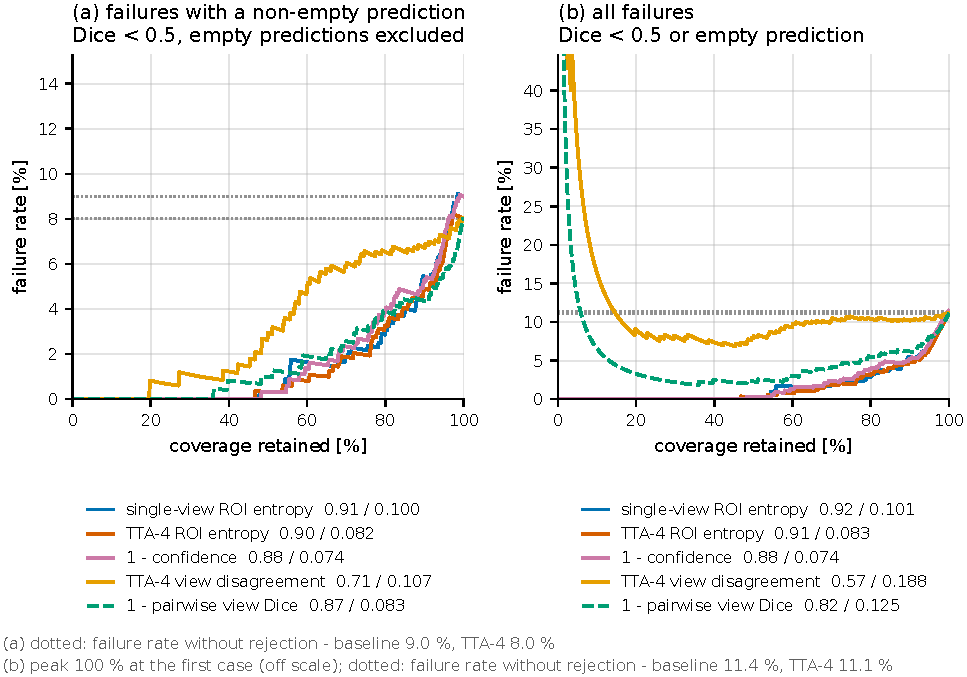
\includegraphics[width=\linewidth]{figures/fig05_risk_coverage.pdf}}
\end{figure}

\begin{figure}[htbp]
\floatconts
  {fig:views}
  {\caption{Change against the single view for 1, 2, 4 and 8 views: (a) Dice, (b) relative HD95 change, for every internal and external setting (colour: dataset; line style and marker: model). Error bars: 95\% bootstrap intervals of the paired per-case change. Small horizontal offsets separate overlapping lines.}}
  {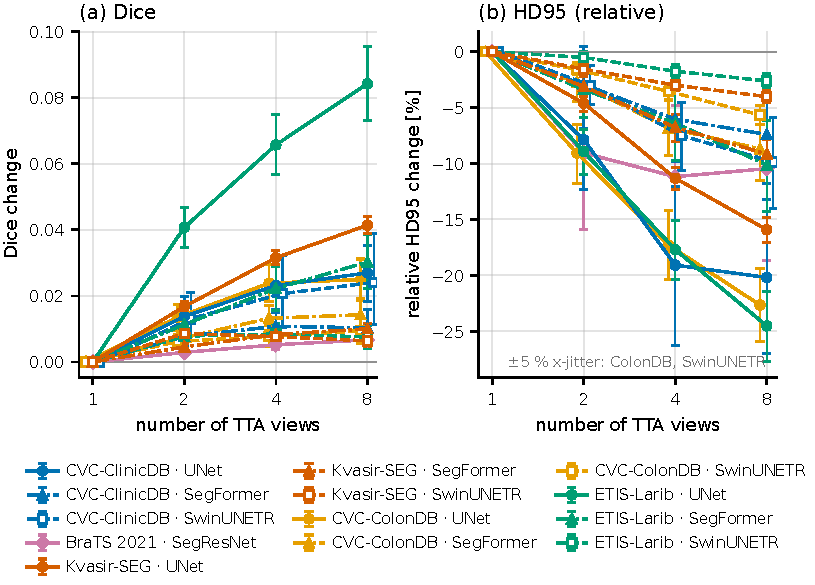
\includegraphics[width=\linewidth]{figures/fig01_gain_vs_views.pdf}}
\end{figure}

\begin{figure}[htbp]
\floatconts
  {fig:ecdf}
  {\caption{ECDF of per-frame HD95 (mean over 3 seeds; frames non-empty under both methods), UNet on CVC-ClinicDB, baseline vs TTA-4. Dashed line: 50\,px; dotted lines: 95th percentiles. Rates printed in the panel exclude empty predictions, so they differ from the text.}}
  {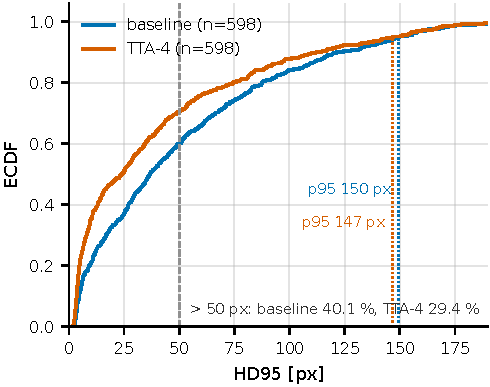
\includegraphics[width=0.6\linewidth]{figures/fig04_hd95_ecdf.pdf}}
\end{figure}

\begin{figure}[htbp]
\floatconts
  {fig:external}
  {\caption{Absolute TTA-8 Dice gain against domain gap, the relative drop of an external collection's baseline Dice below the architecture's internal frame-level baseline. Points at zero gap and dashed lines: internal CVC-ClinicDB gains. These internal gains are frame-level TTA-8 means (UNet 0.028, SwinUNETR 0.021, SegFormer 0.011), not the video-level TTA-4 values of Table~\ref{tab:internal}, so they do not match that table. Error bars: 95\% cluster bootstrap intervals (one image per cluster externally, one video internally).}}
  {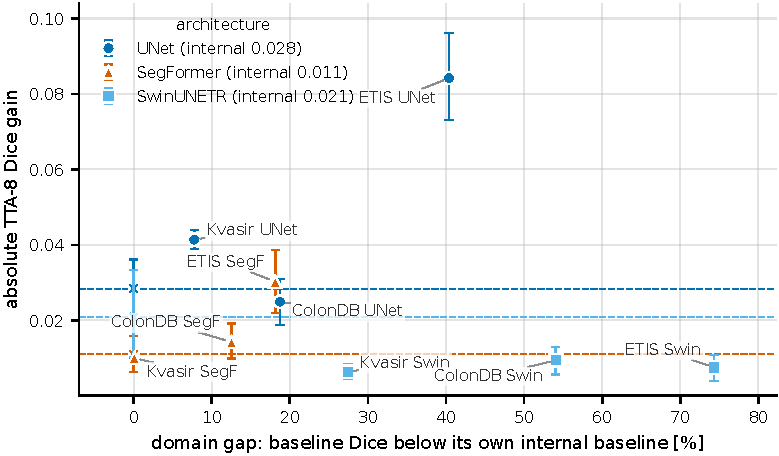
\includegraphics[width=\linewidth]{figures/fig02_internal_vs_external.pdf}}
\end{figure}


\paragraph{The single-view detection curve.} The three comparable rates of Section~\ref{sec:res-rules} in full. At the single view's false-alarm rates of 70.8\%, 75.6\% and 84.8\% ($t=0.5$, 0.4, 0.3), its share of empty predictions over image-checkpoint pairs on CVC-ColonDB and ETIS-Larib was 11.7\%, 10.5\% and 7.2\%, against 11.3\%, 9.9\% and 6.6\% for TTA-8 linearly interpolated between its neighbouring thresholds at those same rates. Counted by a majority of checkpoints the order reverses at two of the three rates and ties at the third: 10.4\%, 9.4\% and 4.3\% against 10.6\%, 9.4\% and 5.0\%. The sweep moves only the empty-versus-non-empty decision; we did not re-threshold non-empty predictions.

\section{Miss counts under different criteria}
\label{app:criteria}
% Source: results/paper_checks/strict_overlap.csv, strict_overlap_transitions.csv, per_checkpoint_spread.csv,
% miss_clustering.csv (scripts/paper_checks/robustness_checks.py).
Table~\ref{tab:criteria} repeats the external counts of Table~\ref{tab:external} for IoU thresholds from 0 (no overlap) to 0.50. A rise that is significant appears only at 0, where all three SwinUNETR counts rise, and at 0.05, where SwinUNETR on Kvasir-SEG still does (125 to 144). From 0.10 upward no count rose significantly for any model on any set. Several fell: for UNet on ETIS-Larib the fall is numerical at 0.05 and significant at every threshold from 0.10 upward, and on Kvasir-SEG it is significant at 0.25 and 0.50. Counted per checkpoint, SwinUNETR's predictions with no overlap rose in all 15 checkpoints on every set (median change $+25$, $+14$ and $+11$ predictions), while its predictions with IoU below 0.10 rose in 10, 8 and 4 checkpoints and fell in 5, 7 and 8 (3 unchanged on ETIS-Larib). For UNet on ETIS-Larib, predictions with IoU below 0.10 fell in all 15 checkpoints (median $-11$). External images carry no sequence labels. As a rough check of independence we grouped the newly affected images into runs of consecutive image numbers and compared the number of runs with random placement (10,000 permutations). The 14 newly empty UNet images on ETIS-Larib formed 9 runs against 13.1 expected ($p=0.001$), and the 27 SwinUNETR images that newly lost overlap on CVC-ColonDB formed 21 runs against 25.2 ($p=0.006$); the 15 newly empty UNet images on CVC-ColonDB formed 15 runs. The 9 ETIS-Larib images that UNet no longer missed under the IoU criterion formed 7 runs against 8.6 expected ($p=0.045$), so they are not fully independent either.

We therefore repeated every external comparison with a block bootstrap. Images are cut into contiguous blocks of consecutive image numbers, with the block length set to the mean sequence length reported for the collection (CVC-ColonDB: 380 images over the 15 sequences its release describes, so 25, although that sequence count belongs to the 300-frame release and not to the 380-frame split we use; ETIS-Larib: 196 in 34, so 6; Kvasir-SEG carries no released sequence labels and we did not block it, so its intervals resample images), and blocks are resampled with replacement 10,000 times. Other bootstrap intervals in this paper use 10,000 draws, reduced to 2,000 for between-model gain comparisons and MC-Dropout and 1,000 for the uncertainty audit and its paired tests. The blocks stand in for sequences; they are not the real ones, real sequences are not of equal length, and on CVC-ColonDB there are only about 15 of them, so the effective sample size is small and these intervals are a sensitivity check rather than a cluster-correct analysis. No conclusion changed, which we read as a sign that the block structure recovers little of the real clustering rather than as evidence that clustering is absent. The intervals of the change exclude zero exactly where the image-level tests were significant: UNet empty predictions $[7, 20]$ on CVC-ColonDB and $[4, 23]$ on ETIS-Larib, SwinUNETR images with no overlap $[15, 36]$, $[16, 37]$ and $[12, 32]$, and the fall in UNet missed images on ETIS-Larib $[-18, -2]$. They include zero everywhere the image-level tests were not significant, including every missed count for SwinUNETR ($[-6, 20]$, $[-21, 7]$ and $[-7, 4]$) and for UNet on CVC-ColonDB ($[-2, 6]$).

\begin{table}[htbp]
\floatconts
  {tab:criteria}%
  {\caption{External images counted as missed by at least 8 of 15 checkpoints, baseline $\rightarrow$ TTA-8, for IoU below the threshold in the column head; 0 means no overlap (Dice $=0$). We swept nine thresholds (0, 0.05, 0.10, 0.15, 0.20, 0.25, 0.30, 0.40, 0.50) and show five here; the four omitted ones are monotone between their neighbours and change no conclusion. $^{\dagger}$exact McNemar $p<0.01$ (unadjusted); the direction is given by the arrow.}}%
  {
  \begin{tabular}{@{}llccccc@{}}
  \toprule
  Data & Model & 0 & 0.05 & 0.10 & 0.25 & 0.50 \\
  \midrule
  \multirow{3}{*}{Kvasir} & UNet & 1$\rightarrow$1 & 9$\rightarrow$8 & 27$\rightarrow$26 & 109$\rightarrow$92$^{\dagger}$ & 310$\rightarrow$250$^{\dagger}$ \\
   & SegFormer & 0$\rightarrow$1 & 5$\rightarrow$5 & 10$\rightarrow$9 & 27$\rightarrow$29 & 120$\rightarrow$113 \\
   & SwinUNETR & 18$\rightarrow$43$^{\dagger}$ & 125$\rightarrow$144$^{\dagger}$ & 216$\rightarrow$223 & 501$\rightarrow$487 & 862$\rightarrow$836$^{\dagger}$ \\
  \midrule
  \multirow{3}{*}{ColonDB} & UNet & 70$\rightarrow$70 & 72$\rightarrow$72 & 74$\rightarrow$76 & 92$\rightarrow$88 & 134$\rightarrow$132 \\
   & SegFormer & 12$\rightarrow$11 & 31$\rightarrow$22 & 36$\rightarrow$33 & 55$\rightarrow$47 & 94$\rightarrow$95 \\
   & SwinUNETR & 73$\rightarrow$99$^{\dagger}$ & 147$\rightarrow$146 & 189$\rightarrow$182 & 279$\rightarrow$278 & 354$\rightarrow$350 \\
  \midrule
  \multirow{3}{*}{ETIS} & UNet & 33$\rightarrow$33 & 47$\rightarrow$40 & 55$\rightarrow$46$^{\dagger}$ & 85$\rightarrow$58$^{\dagger}$ & 131$\rightarrow$89$^{\dagger}$ \\
   & SegFormer & 8$\rightarrow$7 & 14$\rightarrow$15 & 17$\rightarrow$16 & 31$\rightarrow$28 & 59$\rightarrow$48$^{\dagger}$ \\
   & SwinUNETR & 50$\rightarrow$71$^{\dagger}$ & 129$\rightarrow$125 & 145$\rightarrow$144 & 170$\rightarrow$171 & 192$\rightarrow$186 \\
  \bottomrule
  \end{tabular}}
\end{table}


\section{Recovery rules in full}
\label{app:rules}

\begin{figure}[!t]
\floatconts
  {fig:operating}
  {\caption{UNet's operating point without TTA, with TTA-4 and TTA-8, and with the recovery rules (markers): false-alarm rate on 1009 polyp-free cecum frames against the share of images left empty by at least 8 of 15 checkpoints on CVC-ColonDB and ETIS-Larib pooled (576 images). Solid line: TTA-8 with thresholds 0.5 to 0.2. Dashed line with open markers: the single view with the same thresholds. SegFormer is not plotted because almost none of its images are empty by majority. Every point sits above 50\% per-frame false alarms, so this compares inference procedures and is not a deployment curve. Missed images are in Table~\ref{tab:rules}.}}
  {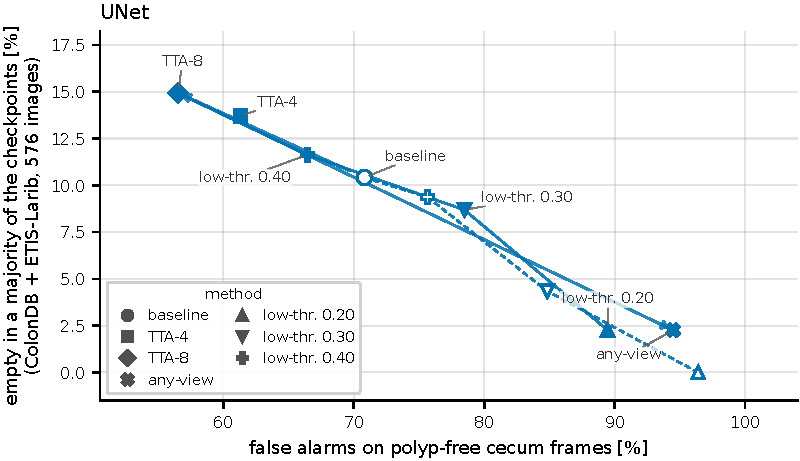
\includegraphics[width=\linewidth]{figures/fig08_operating_point.pdf}}
\end{figure}


Section~\ref{sec:res-rules} reports these numbers in the text. The rules are a probe into the shape of the trade-off and not a deployable setting: both fire on 90\% or more of polyp-free frames.

\begin{table}[htbp]
\floatconts
  {tab:rules}%
  {\caption{Empty predictions, missed images and false alarms, UNet (CVC) and SegResNet (BraTS). The rules are applied to TTA-8, and in the last row to the single view ($-$ = not run). Empty: majority of checkpoints (external), $\geq$2 of 3 seeds (internal), per patient (BraTS). Missed (IoU $<0.10$): majority of checkpoints. False alarms: share of 1009 polyp-free HyperKvasir cecum frames with a non-empty prediction (mean over 15 checkpoints); BraTS: patients of 33 without enhancing tumour (ET-free) with any predicted enhancing tumour. $^{*}$The threshold $t$ was chosen on these data (in-sample).}}%
  {
  \begin{tabular}{@{}lcccccccc@{}}
  \toprule
  Method & \multicolumn{4}{c}{Empty} & \multicolumn{2}{c}{Missed} & \multicolumn{2}{c}{False alarms} \\
  \cmidrule(lr){2-5}\cmidrule(lr){6-7}\cmidrule(lr){8-9}
   & CVC & ColonDB & ETIS & BraTS & ColonDB & ETIS & Cecum & BraTS \\
   & (612) & (380) & (196) & (1218) & (380) & (196) & frames & (33) \\
  \midrule
  Baseline            & 15 & 55 & 5  & 6 & 74 & 55 & 70.8\% & 22 \\
  TTA-8               & 19 & 68 & 18 & 7 & 76 & 46 & 56.5\% & 21 \\
  Any-view            & 5  & 13 & 0  & 0 & 52 & 42 & 94.5\% & 32 \\
  Low-thr. 0.20       & 8$^{*}$ & 13 & 0 & 0 & 65 & 41 & 89.5\% & 30 \\
  Low-thr. 0.30       & 14 & 45 & 5 & 3 & 71 & 44 & 78.5\% & 27 \\
  Low-thr. 0.40       & 17 & 53 & 14 & 5 & 73 & 46 & 66.4\% & 24 \\
  Single view 0.20    & $-$ & 0 & 0 & $-$ & 73 & 55 & 96.4\% & $-$ \\
  \bottomrule
  \end{tabular}}
\end{table}

\section{Lesion-size subgroups}
\label{app:size}
% Source: external_by_model/subgroup_delta.csv, subgroup_interaction.csv, subgroup_summary.csv (TTA-8 vs baseline).
For UNet, the TTA-8 Dice gain differed between size tertiles on all three external collections (Kruskal--Wallis, Holm $p\leq0.03$). On Kvasir-SEG it fell with polyp size (0.061, 0.040 and 0.023 from the smallest to the largest tertile), and on CVC-ColonDB the gain for the largest polyps was small (0.005, 95\% CI $[-0.007, 0.016]$). SwinUNETR lost Dice on the largest polyps of Kvasir-SEG and CVC-ColonDB ($-0.003$ and $-0.008$). SegFormer's gain did not differ between tertiles on CVC-ColonDB or ETIS-Larib (Holm $p=1.0$). The images left empty by most UNet checkpoints rose in every tertile: on CVC-ColonDB from 23 to 30, 12 to 13 and 20 to 25 in the small, medium and large tertiles, and on ETIS-Larib from 4 to 10, 1 to 5 and 0 to 3 (counts, not tested per tertile; Section~\ref{sec:res-external}); SwinUNETR left no image empty by majority in any tertile (Fig.~\ref{fig:size}).
\begin{figure}[htbp]
\floatconts
  {fig:size}
  {\caption{Size tertiles of reference polyp area, cut per external collection (Kvasir-SEG at 25{,}204 and 55{,}261\,px; CVC-ColonDB at 7{,}471 and 16{,}726\,px; ETIS-Larib at 13{,}723 and 49{,}260\,px). Top: TTA-8 Dice gain with 95\% bootstrap intervals for (a) UNet, (b) SegFormer and (c) SwinUNETR. Bottom: share of images left empty by at least 8 of 15 checkpoints without TTA (open markers) and with TTA-8 (filled).}}
  {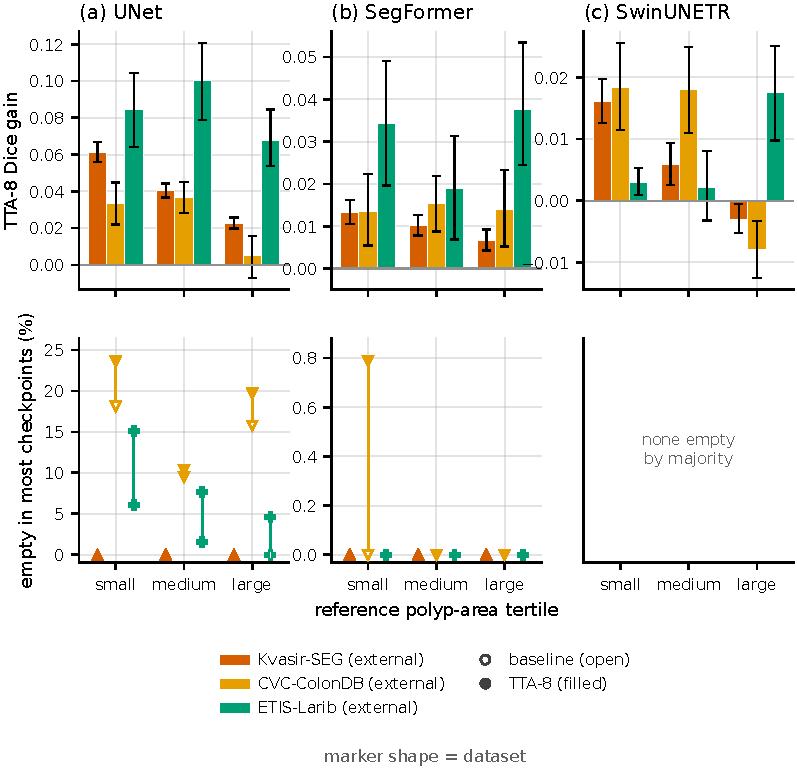
\includegraphics[width=\linewidth]{figures/fig06_size_subgroups.pdf}}
\end{figure}

\section{Qualitative examples}
\label{app:qualitative}
% Source: scripts/figures/fig07_qualitative.py (selection rule, recomputation, Dice assertion).
Rows in Fig.~\ref{fig:qualitative} were chosen by a fixed rule, not by eye. An external row qualifies when most of the 15 checkpoints give a non-empty prediction without TTA and most give an empty one with TTA-8. The internal rows are the two CVC-ClinicDB frames with the largest TTA-4 Dice gain averaged over seeds. The maps of each row were recomputed with the stated checkpoint through the evaluation code, and the Dice printed for each row was checked against the evaluation table (tolerance 0.011).

\begin{figure}[htbp]
\floatconts
  {fig:qualitative}
  {\caption{Top three rows: external polyps (CVC-ColonDB, ETIS-Larib) on which most of the 15 checkpoints give a non-empty prediction without TTA and most an empty one with TTA-8. Bottom two rows: internal CVC-ClinicDB frames with the largest TTA-4 Dice gain averaged over seeds, each drawn with the checkpoint showing the largest gain. External rows are drawn with a checkpoint in which the TTA-8 prediction is empty and the baseline Dice is at least 0.3, smallest polyps first; the Dice of each row is printed next to it. The external rows show individual losses, which are the minority among newly empty images; Table~\ref{tab:external} gives net counts.}}
  {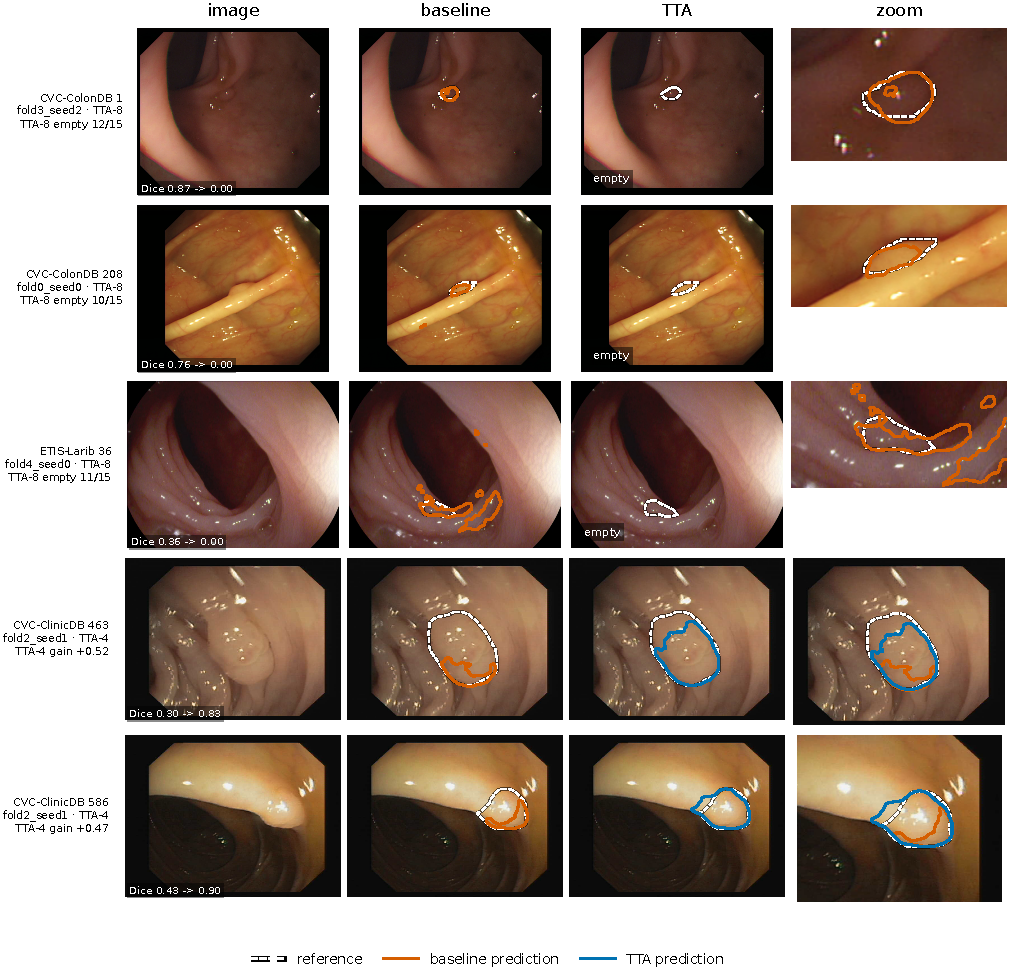
\includegraphics[width=\linewidth]{figures/fig07_qualitative.pdf}}
\end{figure}

\section{False alarms on polyp-free frames}
\label{app:sanity}
% Source: scripts/figures/sanity_false_alarms.py (seeded draw, CPU recomputation, region attribution,
% preprocessing assertion against the Kvasir-SEG loader).
To rule out a pipeline artefact behind the high false-alarm rates, we drew baseline false alarms at random (fixed seed) from the fold-0, seed-0 UNet and SegFormer runs, recomputed them on the CPU through the evaluation code, and assigned every predicted region to what it covers: mucosa, the black border, the endoscope overlay box or the overlay text. All twelve shown lie on mucosa (Fig.~\ref{fig:sanity}). A numerical check confirmed that the polyp-free frames pass through the same preprocessing as Kvasir-SEG, giving the same network input for the same image file.

\begin{figure}[htbp]
\floatconts
  {fig:sanity}
  {\caption{Twelve baseline false alarms on HyperKvasir normal cecum frames, drawn at random with a fixed seed from one checkpoint pair (fold 0, seed 0): eight UNet (blue) and four SegFormer (vermillion). All twelve lie on mucosa, none on the overlay box, border or text.}}
  {\includegraphics[width=\linewidth]{figures/sanity_false_alarms.png}}
\end{figure}

\section{Effects per 1000 cases and latency}
\label{app:deployment}
% Source: aggregate_*/tail_metrics.csv and detection_seed_averaged.csv (internal), results/paper_checks/
% brats_tail_et_only.csv (BraTS, 1218 ET patients), external_by_model/misses.csv (external, majority of 15
% checkpoints), deployment_terms/pass_latency.csv (2D latency). No BraTS latency: no measurement record.
Table~\ref{tab:deployment} restates the main effects per 1000 cases. Large failures fixed is the drop in the share of cases with HD95 above 50\,px (CVC-ClinicDB) or 10\,mm (BraTS) or with no prediction. Empty added is the net change in empty cases, by majority of seeds (internal) or of the 15 checkpoints (external). SwinUNETR lost all overlap on 25, 68 and 107 more images per 1000 on Kvasir-SEG, CVC-ColonDB and ETIS-Larib, but by the IoU criterion no model missed significantly more images (Table~\ref{tab:criteria}). Latency is estimated as the number of views times the measured median per-pass time.

\begin{table}[htbp]
\floatconts
  {tab:deployment}%
  {\caption{Effects per 1000 cases and estimated latency per image (-- = not measured). External settings not listed added no empty predictions by majority (Kvasir-SEG for every model; SegFormer on ETIS-Larib; SwinUNETR everywhere).}}%
  {
  \begin{tabular}{lcccccc}
  \toprule
  Setting & \multicolumn{2}{c}{Large failures fixed} & \multicolumn{2}{c}{Empty added} & \multicolumn{2}{c}{Latency (ms)} \\
  \cmidrule(lr){2-3}\cmidrule(lr){4-5}\cmidrule(lr){6-7}
   & TTA-4 & TTA-8 & TTA-4 & TTA-8 & 1 view & TTA-8 \\
  \midrule
  UNet, CVC-ClinicDB        & 99.7 & 111.1 & 6.5 & 6.5 & 37 & 298 \\
  SegFormer, CVC-ClinicDB   & 21.2 & 21.2  & 0.0 & 0.0 & 87 & 694 \\
  SwinUNETR, CVC-ClinicDB   & 47.4 & 65.4  & 0.0 & 0.0 & 73 & 580 \\
  SegResNet, BraTS (ET)     & 12.3 & 15.6  & 2.5 & 0.8 & -- & -- \\
  UNet, CVC-ColonDB         & --   & --    & 21.1 & 34.2 & 37 & 298 \\
  UNet, ETIS-Larib          & --   & --    & 56.1 & 66.3 & 37 & 298 \\
  SegFormer, CVC-ColonDB    & --   & --    & 2.6 & 2.6 & 87 & 694 \\
  \bottomrule
  \end{tabular}}
\end{table}

\section{Reproducibility}
\label{app:repro}

\paragraph{CVC-ColonDB counts.} Sources disagree on this collection. Its release describes 15 sequences from 15 studies and annotates 300 frames \cite{bernal2012colondb}; later descriptions report 13 sequences from 13 patients \cite{vazquez2017endoscene,tudela2024benchmark}; and the PraNet test split we use contains 380 frames. We could not establish how the extra frames were added, so we report the split as distributed and treat its 380 frames as the evaluation population.
\paragraph{Software and hardware.} All runs used Python 3.13.7, PyTorch 2.6.0 (CUDA 12.4, cuDNN 9.1), MONAI 1.5.2, segmentation-models-pytorch 0.5.0 and NumPy 2.4.1 on Windows 11, with deterministic algorithms enabled, as recorded in each run file. Exact versions are pinned in \texttt{requirements.txt} in the repository. Training and evaluation ran on one NVIDIA RTX 4050 laptop GPU (6\,GB); the 15 runs that recomputed pairwise view Dice ran on the CPU. Deterministic algorithms and fixed seeds make a run reproducible on the same hardware and library versions, but not bitwise across different GPUs or driver versions.

\paragraph{Seeds and runs.} The 2D seeds are 0, 1 and 2, crossed with folds 0 to 4, giving the 15 checkpoints per architecture; the MC-Dropout grid uses the same 15 pairs, and the data sweep and the 3D SegResNet use seed 0 only with 5 folds each. Each seed is set globally for Python, NumPy and PyTorch at the start of a run. The BraTS configuration is the reduced SegResNet of \texttt{configs/brats2021/segresnet\_reduced.yaml}, which lowers the initial filter count to fit the 6\,GB GPU.

\paragraph{Code and data.} Code, configurations, split files and all result tables are at \url{https://github.com/Subkash2206/worse-where-it-matters}, with a README describing how each table and figure is regenerated from the committed results. Trained weights are not distributed because of their size: every number downstream of the committed result tables can be recomputed without retraining, while reproducing the tables themselves requires rerunning the grids with the seeds above. No image data are redistributed. CVC-ClinicDB, Kvasir-SEG, HyperKvasir, CVC-ColonDB and ETIS-Larib are public downloads; BraTS 2021 requires registration with the challenge organisers.
